% Design

% Design Equations and specs to find G(s)
The specifications given for the filter are used in are as follows:

\begin{align*}
A_{max} &= 1 \, dB\\
A_{min} &= 20 \, dB\\
f_c &= 25 \, kHz\\
f_s &= 50 \, kHz\\
5 &\le K_o \le 10\\
\end{align*}

where $A_{max}$ is the maximum passband attenuation, $A_{min}$ is the minimum stopband attenuation, $f_c$ is the passband edge frequency, $f_s$ is the stopband edge frequency, and $K_o$ is the DC gain. These values were used with the following Butterworth filter design equations in order to determine the minimum filter order $N$ and the poles $p_k$\cite{fdesign}:

\begin{equation}\label{eq:buttdesign}
\left( \dfrac{\omega_s}{\omega_c} \right)^{2N} \ge \dfrac{10^{0.1A_{min}} - 1}{\epsilon^2}
\end{equation}

where the parameter $\epsilon$ is given by

\begin{align*}
\epsilon &= \sqrt{10^{0.1A_{max}-1}}\\
&= 0.5088
\end{align*}

The minimum $N$ for which Equation \ref{eq:buttdesign} is satisfied was then determined:

\begin{align*}
\left( \dfrac{2\pi(50\,kHz)}{2\pi(25\,kHz)} \right)^{2N} &= \dfrac{10^{0.1(20)} - 1}{0.5088^2}\\
2^{2N} &= 382.4203 \\
N &\ge 4.29 \\
N &= 5
\end{align*}

Then, the $N=5$ poles $p_k$ are distributed on a circle of radius $\omega_o$ where $\omega_o$ is given by the following:

\begin{align*}
\omega_o &= \omega_c \left( \dfrac{1}{\epsilon}  \right) ^{1/N}\\
&= 2\pi(25\,kHz) \left( \dfrac{1}{0.5088}  \right) ^{1/5}\\
&= 1.798 \times 10^5 rad/s
\end{align*}

Then, the poles are given by the following:

\begin{align*}
p_k &= \omega_o \left[ -\sin{\left(\dfrac{(2k-1)\pi}{2N}\right) } + j\cos{\left(\dfrac{(2k-1)\pi}{2N}\right)} \right],\quad 1\le k \le N \\
p_{(1,5)} &= (-0.556 \pm j1.71) \times 10^5\\
p_{(2,4)} &= (-1.455 \pm j1.06) \times 10^5\\
p_{(3)} &= -1.798 \times 10^5
\end{align*}

The overall transfer function $G(s)$ is given by

\begin{align*}
G(s) &= \dfrac{K_o \omega_o^N}{(s-p_1)(s-p_2)\ldots(s-p_5)}\\
\end{align*}
and
\begin{align*}
G(s) &= \dfrac{K_o\, 1.88 \times 10^{26}}{s^5 + 5.82\times 10^5 s^4 + 1.69\times 10^{11} s^3 + 3.04\times 10^{16} s^2 + 3.38\times 10^{21} s + 1.88 \times 10^{26}}\\
\end{align*}

% Verifying that G(s) meets the specification as given
As a check, this transfer function's magnitude response was plotted in MATLAB to make sure that it met the specifications for the filter. Because $K_o$ can be set easily, it was assumed to be 1 for this simulation. The theoretical magnitude response is plotted against the specification in Figure \ref{fig:theo}.

\begin{figure}[H]
\centering
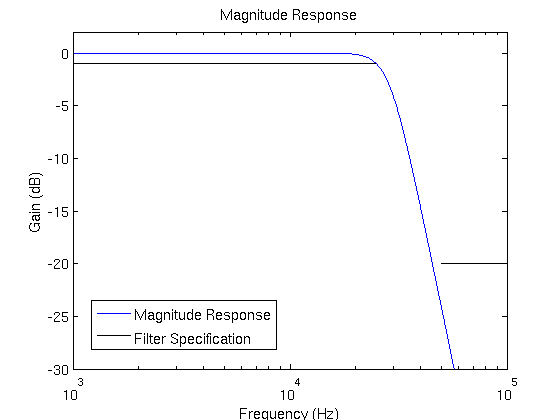
\includegraphics[scale=.75]{fig/mag_theo.png}
\caption{Theoretical Magnitude Response for G(s)\label{fig:theo}}
\end{figure}

% Splitting the xfcn into sections and choosing component values
From here, the transfer function $G(s)$ was split into two second-order subsystems and a first-order system as a cascade\cite{tfnotes}. This makes the system realizable since the whole transfer function is not practically implemented as one system. From the poles $p_k$, the two complex conjugate pairs form the two standard second-order subsystems, and the real pole was implemented as a first-order subsystem. Then, a last inverting gain stage is added to vary the DC gain as well as
invert the phase to maintain the proper phase, impulse, and step responses. The subsystem transfer functions are then given by the following:

\begin{align*}
G(s) &= G_1(s)G_2(s)G_3(s)G_4(s)\\
G_1(s) &= -\dfrac{G_{l1}\omega_o}{s+\omega_o}\\
G_2(s) &= -\dfrac{G_{l2}\omega_o^2}{s^2+2\zeta_2 \omega_o s + \omega_o^2}\\
G_3(s) &= -\dfrac{G_{l3}\omega_o^2}{s^2+2\zeta_3 \omega_o s + \omega_o^2}\\
G_4(s) &= -K_o
\end{align*}

where $\zeta_2=0.309$, $\zeta_3=0.809$, and the lowpass DC gains are given by $G_l$. 

A simulation diagram illustrating the system is given in Figure \ref{fig:sim}. From this, the complete system was realized as shown in the schematic diagram in Figure \ref{fig:ckt}. 

\begin{figure}[H]
\centering
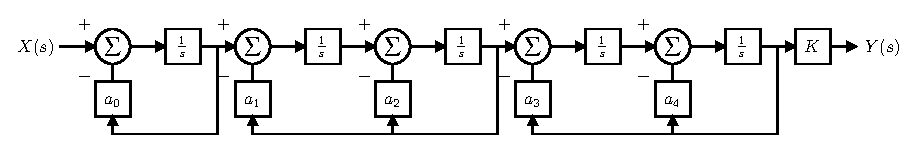
\includegraphics[width=\textwidth]{fig/simdiag}
\caption{Simulation Diagram for G(s)\label{fig:sim}}
\end{figure}

\begin{figure}[H]
\centering
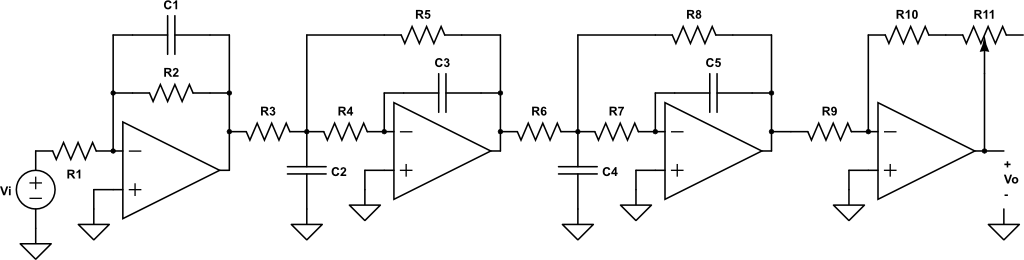
\includegraphics[width=\textwidth]{fig/ckt.png}
\caption{Schematic Diagram for Butterworth Filter with Variable Gain\label{fig:ckt}}
\end{figure}

Capacitors were first selected when choosing component values. Then, using the subsystem transfer functions, the resistor values were determined. The component values used are summarized in Table \ref{tbl:comp}.

\begin{table}[H]
\centering
\begin{tabular}{|c|c|c|c|}
\hline
Component & Value & Component & Value\\ \hline\hline
$R_1$ & $12.2\,k\Omega$ & $R_6$ & $455\,\Omega$ \\ \hline
$R_2$ & $5.57\,k\Omega$ & $R_7$ & $20\,k\Omega$ \\ \hline
$C_1$ & $1\,nF$ & $R_8$ & $1.547\,k\Omega$ \\ \hline
$R_3$ & $2.42\,k\Omega$ & $C_4$ & $10\,nF$ \\ \hline
$R_4$ & $20\,k\Omega$ & $C_5$ & $68\,pF$ \\ \hline
$R_5$ & $1.547\,k\Omega$ & $R_9$ & $5.1\,k\Omega$ \\ \hline
$C_2$ & $10\,nF$ & $R_{10}$ & $5.1\,k\Omega$ \\ \hline
$C_3$ & $115\,pF$ & $R_{11}$ & $0-100\,k\Omega$ \\ \hline
\end{tabular}
\caption{Component Values for Butterworth Filter\label{tbl:comp}}
\end{table}
% Comp table for presentation
%\begin{table}[H]
%\centering
%\begin{tabular}{|c|c|c|c|c|c|c|c|}
%\hline
%Component & Value & Component & Value & Component & Value & Component & Value\\ \hline\hline
%$R_1$ & $12.2\,k\Omega$ & $R_4$ & $20\,k\Omega$ & 		$R_6$ & $455\,\Omega$ &$C_5$ & $68\,pF$ \\ \hline 
%$R_2$ & $5.57\,k\Omega$ & $R_5$ & $1.547\,k\Omega$ & $R_7$ & $20\,k\Omega$ & $R_9$ & $5.1\,k\Omega$ \\ \hline
%$C_1$ & $1\,nF$ & 			     $C_2$ & $10\,nF$ & 				$R_8$ & $1.547\,k\Omega$ & $R_{10}$ & $5.1\,k\Omega$ \\ \hline
%$R_3$ & $2.42\,k\Omega$ & $C_3$ & $115\,pF$ & 				 $C_4$ & $10\,nF$ & $R_{11}$ & $0-100\,k\Omega$ \\ \hline
%\end{tabular}
%\caption{Component Values for Butterworth Filter\label{tbl:comp}}
%\end{table}


% Verify that slightly modified xfcn still meets the spec as given
To see how well each subsystem was realized, its transfer function is evaluated for the values of the components used in order to see any deviations in the natural frequency $\omega_o$, pole values $p_k$, and damping factor $\zeta$. 

For the first subsystem,

\begin{equation*}
G_1(s) = -\dfrac{G_{l1}\omega_o}{s+p_1}
\end{equation*}

where

\begin{align*}
G_{l1}\omega_o &= \dfrac{1}{R_1C_1}\\
&= 8.197 \times 10^4\\ % = 0.456\omega_o = 8.199\times 10^5 \\
G_{l1} &= 0.457
\end{align*}

and

\begin{align*}
p_1 &= \dfrac{1}{R_2C_1}\\
&= 1.795\times 10^5 \\
&\approx \omega_o %= 1.798\times 10^5 \\
\end{align*}

For the second subsystem,

\begin{equation*}
G_2(s) = -\dfrac{G_{l2}\omega_{n2}^2}{s^2+2\zeta_2\omega_{n2} s + \omega_{n2}^2}
\end{equation*}

where

\begin{align*}
\omega_{n2} &= \dfrac{1}{\sqrt{R_4R_5C_2C_3}}\\
&= 1.68 \times 10^5 \\
&\approx 0.9 \omega_o\\
\zeta_2 &= \dfrac{1}{2C_2\omega_{n2}}\left(\dfrac{1}{R_3}+\dfrac{1}{R_5}+\dfrac{1}{R_5}\right)\\
&= 0.3302 \\
&\approx 1.1\zeta_2
\end{align*}
and
\begin{align*}
G_{l2} &= \dfrac{R_5}{R_3}\\
&=0.639
\end{align*}

For the third subsystem,

\begin{equation*}
G_3(s) = -\dfrac{G_{l3}\omega_{n3}^2}{s^2+2\zeta_3\omega_{n3} s +z \omega_{n3}^2}
\end{equation*}
where
\begin{align*}
\omega_{n3} &= \dfrac{1}{\sqrt{R_7R_8C_4C_5}}\\
&= 2.18 \times 10^5 \\
&\approx 1.2 \omega_o\\
\zeta_3 &= \dfrac{1}{2C_4\omega_{n3}}\left(\dfrac{1}{R_6}+\dfrac{1}{R_7}+\dfrac{1}{R_8}\right)\\
&= 0.664 \\
&\approx 0.82\zeta_3
\end{align*}
and
\begin{align*}
G_{l3} &= \dfrac{R_8}{R_6}\\
&=3.40
\end{align*}

As desired, the magnitude of the DC gain before the fourth inverting gain stage is connected should be given by

\begin{align*}
G_{DC} &= G_{l1}G_{l2}G_{l3}\\
&=0.993\\
&\approx 1 \\
\end{align*}

When the system was first constructed with matched values for the natural frequency $\omega_n$ and $\zeta$ from the initial design equations, the system did not meet the filter specification. The values for capacitance were slightly altered in order to meet the specification by raising $C_3$ from 100pF to 115pF and lowering $C_5$ from 100pF to 68pF. As a design decision, meeting the specification was more important than ensuring that the natural frequency for each subsystem
was exactly the same. This discrepancy in values for $\zeta$ and $\omega_o$ are thus acceptable. However, we should expect our experimental results to show that the passband response is not monotonically decreasing as frequency increases. There could be one or two slight increases in in the magnitude response in the passband near the natural frequency.

For the fourth subsystem, since the potentiometer sweeps from 0-100 $k\Omega$, we expect a gain to range between

\begin{align*}
G_{DC_{min}} &= \dfrac{5.1k\Omega+0}{5.1k\Omega}\\
&= 1\\
G_{DC_{max}} &= \dfrac{5.1k\Omega+100k\Omega}{5.1k\Omega}\\
&= 20.6 \\
\end{align*}

which should satisfy the requirement that the DC gain be between 5 and 10.
